\section{Fundamental concepts}

\subsection{Threat modeling}

\begin{frame}
  \frametitle{What is threat modeling?}
  \begin{itemize}
    \item Threat modeling is the process of listing and organizing potential
      threats and appropriate responses
    \item Helps to:
      \begin{itemize}
        \item Identify potential threats
        \item Prioritize them based on the risk
        \item Identify possible countermeasures
      \end{itemize}
    \item Provides an analysis of what affects the security and which measures
      need to be implemented
    \item A large number of framworks and methodologies exist.
  \end{itemize}
\end{frame}

\begin{frame}
  \frametitle{Security properties: CIA triad}
  \begin{itemize}
    \item \textbf{Confidentiality}:
          Can an unauthorized entity gain access to information?
    \item \textbf{Integrity}:
          Can there be unauthorized modification of information?
    \item \textbf{Availability}:
          Can authorized access to information be impended?
  \end{itemize}
\end{frame}

\begin{frame}
  \frametitle{Confidentiality}
  \begin{itemize}
    \item The main property one wants out of a secure information system
    \item Typical adversary: \textbf{passive} MITM
    \item Protecting it is \textbf{encryption}'s main role
    \item Can make it harder to ensure \textbf{Availability}
  \end{itemize}
\end{frame}

\begin{frame}
  \frametitle{Integrity}
  \begin{itemize}
    \item Aims to ensure that information is not modified
    \item Typical adversary is an \textbf{active} MITM
    \item The most basic form of protection are checksums
  \end{itemize}
\end{frame}

\begin{frame}
  \frametitle{Availability}
  \begin{itemize}
    \item Aims to ensure that information is accessible
    \item Typical adversaries are DoS attacks
    \item Defense usually involves:
    \begin{itemize}
      \item early detection of threats
      \item redundancy and failover
    \end{itemize}
    %% An example here are the "CEO scams", where an authority person
    %% pretends to be offsite/in a meeting/visiting a client and unable
    %% to go through normal procedure, but absolutely needs X to happen NOW
    \item Maintaining availability can lead to compromising on confidentiality,
          this is what some scams rely on.
  \end{itemize}
\end{frame}

\begin{frame}
  \frametitle{In cybersecurity: the five pillars}
  \begin{itemize}
    \item \textbf{Confidentiality}:
          Can an unauthorized entity gain access to information?
    \item \textbf{Integrity}:
          Can there be unauthorized modification of information?
    \item \textbf{Availability}:
          Can authorized access to information be impended?
    \item \textbf{Authenticity}:
          Can an unauthorized entity insert undistinguishable information?
    \item \textbf{Non-repudiation}:
          Can an authorized entity deny some information's authenticity?
  \end{itemize}
  %% Not particularly useful, imho. I prefer CIAAN.
  The \textbf{Parkerian hexad} introduces
  \begin{itemize}
    \item \textbf{Utility}:
          Is the information useful?
  \end{itemize}
  and trades \textbf{Non-repudiation} for
  \begin{itemize}
    \item \textbf{Control}:
          Can authorized users access information?
  \end{itemize}
\end{frame}

\begin{frame}
  \frametitle{Authenticity}
  \begin{itemize}
    \item Aims to ensure that information (e.g.) a message came from a source
    \item This is what digital signatures aim to protect
    \item This is not the same as integrity:
    \begin{itemize}
      \item No protection against \textbf{replaying} a signed message
    \end{itemize}
  \end{itemize}
\end{frame}

\begin{frame}
  \frametitle{Non-repudiation}
  \begin{itemize}
    \item Ensures that actions or messages cannot be disavowed after the fact
    \item Properly implemented digital signature schemes can protect it
    \item Precise context must be included in the signature to be effective
  \end{itemize}
\end{frame}


\begin{frame}
  \frametitle{Threat modeling frameworks: STRIDE}
  Flip side of the security properties:
  \begin{itemize}
    \item \textbf{Spoofing}: Unauthorized use of credentials
    \item \textbf{Tampering}: Unauthorized modification of information
    \item \textbf{Repudiation}: Performing unauthorized actions that cannot be detected
    \item \textbf{Information disclosure}: Unauthorized access to information
    \item \textbf{Denial of Service}: Disruption of authorized access to a resource
    \item \textbf{Elevation of privilege}: Execution of unauthorized actions
  \end{itemize}
\end{frame}

\begin{frame}
  \frametitle{Threat modeling frameworks: Attack tree}
  \begin{itemize}
    \item Popularized by \href{https://www.schneier.com/academic/archives/1999/12/attack_trees.html}{Bruce Schneier}
    \item Start with a goal, e.g. "run a program as root", this is your root node
    \item Children are ways to achieve this goal
    \begin{itemize}
      \item recover root password
      \item elevate local user privilege
      \item make a sudoer run your program as root
      \item replace a setuid binary on the filesystem
    \end{itemize}
    \item Children can then have children themselves
    \item Attribute a cost to leaves, the cost of the parent is the min
  \end{itemize}
\end{frame}

\begin{frame}
  \frametitle{Threat modeling frameworks: \href{https://linddun.org/}{LINDDUN}}
  \begin{itemize}
    \item Privacy-focused threat model
    \item Developed by researchers at KU Leuven
    \item Suitable for GDPR/HIPAA/
    \begin{itemize}
      \item \textbf{Linkability} Can an adversary link actions or data to a person?
      \item \textbf{Identifiability} Can an adversary leak a person's identity?
      \item \textbf{Non-repudiation} Can an adversary attribute a claim to an person?
      \item \textbf{Detectability} Can an adversary detect a person's involvment?
      \item \textbf{Disclosure of information} Can an adversary access personal data?
      \item \textbf{Unawareness} Do persons know how their data is being processed?
      \item \textbf{Non-compliance} Does the system comply with standards and regulation?
    \end{itemize}
  \end{itemize}
\end{frame}

\begin{frame}
  \frametitle{Threat modeling frameworks: PASTA}
  \begin{itemize}
    \item Process for Attack Simultation and Threat Analysis
    \item Rather complex
    \item Works in 7 stages:
    \begin{itemize}
      \item \textbf{Definition of objectives}
      \item \textbf{Definition of technical scope}
      \item \textbf{System decomposition}
      \item \textbf{Threat analysis}
      \item \textbf{Vulnerability analysis}
      \item \textbf{Attack modeling}
      \item \textbf{Impact analysis}
    \end{itemize}
  \end{itemize}
\end{frame}

\begin{frame}
  \frametitle{Which methodology to choose?}
  \begin{itemize}
    \item It is not necessary to follow one
    \item Any Threat Model is better than no Threat Model
    \item These frameworks are mnemonic devices:
    \begin{itemize}
      \item A Threat Model helps to be exhaustive
      \item The one forgotten threat might be the one that is exploited
      \item But they also help define scope
    \end{itemize}
    \item Try one, and adapt it to your needs
  \end{itemize}
\end{frame}

\subsection{Cryptography basics}

\begin{frame}
  \frametitle{Cryptography basics}
  \begin{itemize}
    \item Various types of algorithms can be used to secure sensitive data
      \begin{itemize}
        \item Cryptographic hash functions produce a message digest
        \item Encryption algorithms allow the transformation of plain-text data into
          unintelligible data
          \begin{itemize}
            \item Symmetric cryptography uses the same key to encrypt and decrypt data
            \item Asymmetric cryptography uses a different key to encrypt and decrypt data
          \end{itemize}
      \end{itemize}
    \item Real world protocols will combine different algorithms from several
      types
  \end{itemize}
\end{frame}

\subsubsection{Cryptographic hash function}

\begin{frame}
  \frametitle{Cryptographic hash function}
  \begin{itemize}
    \item Hash functions map data of arbitrary size to a known-size digest
    \item Cryptographic hash functions are suited for cryptographic operations:
      \begin{itemize}
        \item Generally used for message authentication, digital signatures or
          password hashing
      \end{itemize}
    \item Specific requirements on cryptographic hash functions:
      \begin{itemize}
        \item Finding an input message that generates a given hash is unfeasible
        \item For random input data, each possible hash is equally probable
        \item Avalanche effect: small changes on the input produce a completely
          different output
      \end{itemize}
    \item Popular algorithms: MD5, SHA-1, Whirlpool, SHA-2, SHA-3 (Keccak).
    \item SHA-2 and SHA-3 are the most suited for new products
      \begin{itemize}
        \item TLS 1.3 mostly uses SHA-256 and SHA-384
      \end{itemize}
  \end{itemize}
  \begin{center}
    \includegraphics[width=.8\textwidth]{slides/security-fundamental-concepts/cryptographic-hash-function.pdf}
  \end{center}

\end{frame}

\subsubsection{Symmetric encryption}

\begin{frame}
  \frametitle{Symmetric encryption}
  \begin{itemize}
    \item Simplest form of encryption
    \item Encryption and decryption algorithms use the same key
    \item Encryption and decryption algorithm may differ
    \item Historical algorithms: Caesar cipher, Enigma machine, ROT13, XOR
    \item Previously popular algorithms: DES, RC4, Blowfish, and Twofish
    \item Nowadays, AES is the most widespread algorithm
  \end{itemize}
  \begin{center}
    \includegraphics[width=.8\textwidth]{slides/security-fundamental-concepts/symmetric_encrypt.pdf}
  \end{center}
\end{frame}

\begin{frame}
  \frametitle{AES: Advanced Encryption Standard}
  \begin{itemize}
    \item NIST specification from 2001
    \item Based on Rijndael algorithm, developed by Joan Daemen and Vincent Rijmen
    \item Block sizes 128 bits
    \item Key sizes of 128, 192, or 256 bits
    \item Used in a virtually all up-to-date protocols relying on symmetric
      encryption
    \item Low RAM and CPU requirements, can easily be hardware accelerated
  \end{itemize}
\end{frame}

\begin{frame}
  \frametitle{Block Cipher Modes of Operation}
  \begin{itemize}
    \item Most symmetric encryption algorithms operate on blocks of a fixed size
      \begin{itemize}
        \item To encrypt longer data, the data must first be split in as many blocks
          as needed
        \item When encrypting multiple blocks with the same key, some randomness must
          be introduced, otherwise input patterns might be identifiable in the output.
          \begin{center}
            
\includegraphics[width=0.1\textwidth]{slides/security-fundamental-concepts/Tux.pdf}
            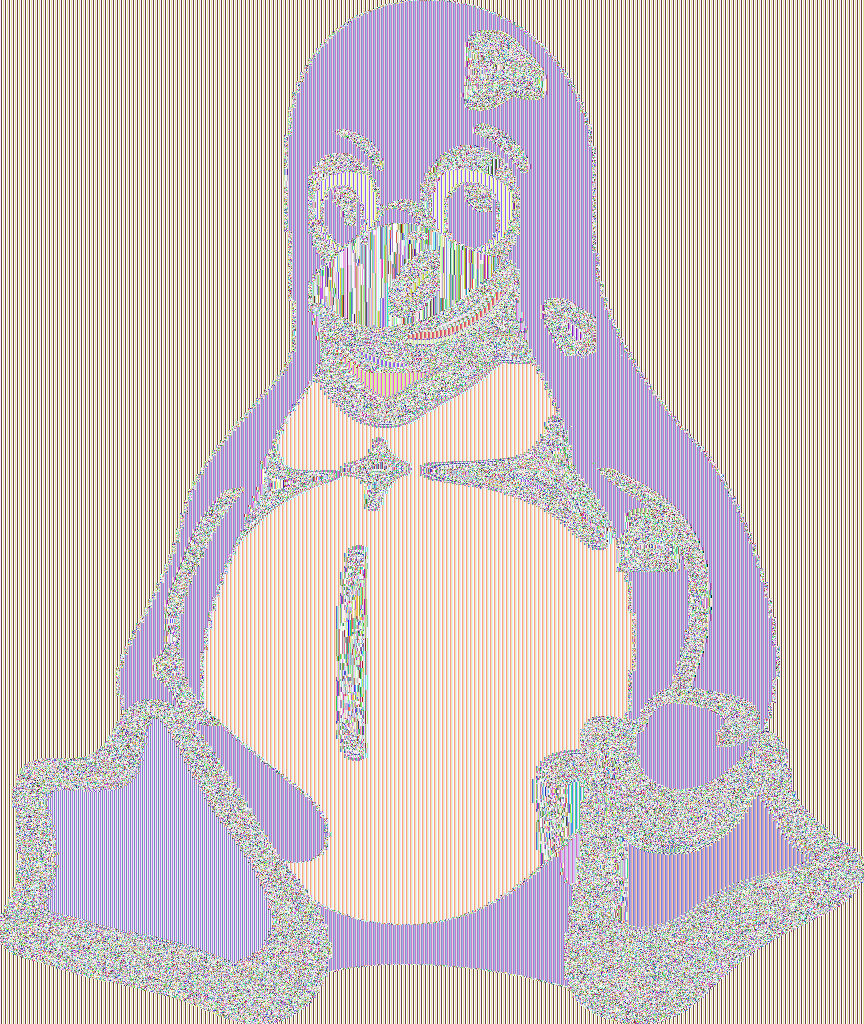
\includegraphics[width=0.1\textwidth]{slides/security-fundamental-concepts/Tux_encrypted_ecb.png}
            \\
            \scriptsize An image and its encryption in ECB mode\\
            \tiny Larry Ewing, Simon Budig, Garrett LeSage, CC0:
            \url{https://en.wikipedia.org/wiki/File:Tux.svg}\\
            \tiny RFL890, CC0:
            \url{https://en.wikipedia.org/wiki/File:Tux_encrypted_ecb.png}\\
          \end{center}
      \end{itemize}
    \item Additionally, we often want protection from data modification by
      third parties and replay attacks
    \item Modes of operation allow to securely chain blocks together
  \end{itemize}
\end{frame}

\begin{frame}
  \frametitle{Block Cipher Modes of Operation Examples (1)}
  \begin{itemize}
    \item Modes ensuring data confidentiality:
      \begin{itemize}
        \item CBC: Cipher block chaining
          \begin{itemize}
            \item Input of each block is XORed with the output of the previous block
            \item The input of the first block is XORed with either a deterministic
              initialization vector or a random one, which is shared along with the
              encrypted data.
          \end{itemize}
        \item CTR: Counter
          \begin{itemize}
            \item An incrementing value is encrypted
            \item This encrypted value is XORed with the input block to generate encrypted data
            \item No dependency between blocks: encryption can be parallelized,
              random blocks can be modified
            \item The initial counter value is derived from a nonce, which
              should be unique for each message encrypted with the same key
          \end{itemize}
      \end{itemize}
  \end{itemize}
  \begin{columns}
    \column{0.5\textwidth}
    \begin{center}
      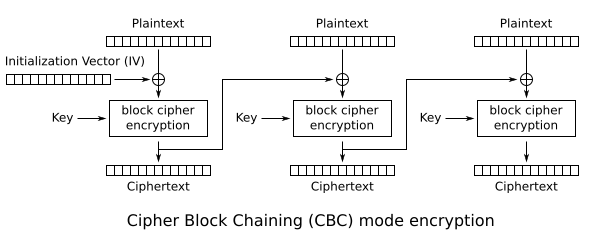
\includegraphics[width=.8\textwidth]{slides/security-fundamental-concepts/CBC_encryption.pdf}
      \tiny WhiteTimberwolf, Public domain: \\\url{https://commons.wikimedia.org/wiki/File:CBC_encryption.svg}\\
    \end{center}
    \column{0.5\textwidth}
    \begin{center}
      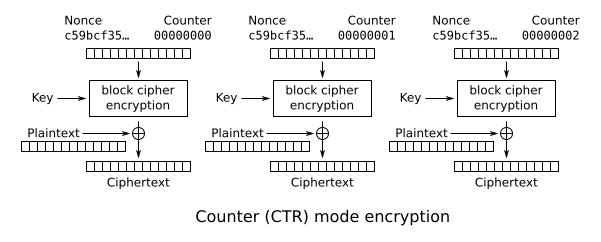
\includegraphics[width=.8\textwidth]{slides/security-fundamental-concepts/CTR_encryption_2.pdf}
      \tiny WhiteTimberwolf, Public domain: \\\url{https://commons.wikimedia.org/wiki/File:CTR_encryption_2.svg}\\
    \end{center}
  \end{columns}
\end{frame}

\begin{frame}
  \frametitle{Block Cipher Modes of Operation Examples (2)}
  \begin{itemize}
    \item Modes ensuring data authentication:
      \begin{itemize}
        \item CBC-MAC: Cipher block chaining message authentication code
          \begin{itemize}
            \item Reuses the CBC mechanism
            \item All blocks are chained: the output of the last block depends on
              all preceding blocks, the key, and the initialization vector
            \item This last block output is the CBC-MAC value
            \item CBC-MAC can be sent with the message, allowing receiver to
              verify data integrity
          \end{itemize}
          \begin{center}
            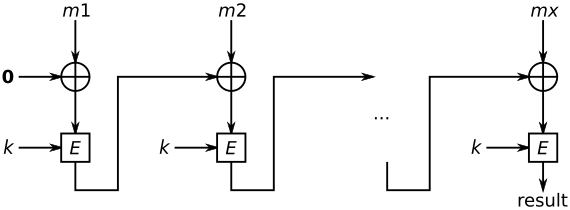
\includegraphics[width=.4\textwidth]{slides/security-fundamental-concepts/CBC-MAC_structure.pdf}\\
            \tiny Benjamin D. Esham, Public domain: \url{https://commons.wikimedia.org/wiki/File:CBC-MAC_structure_(en).svg}\\
          \end{center}
        \item In most situations, keys should not be reused between confidentiality
          and authentication modes, at the risk of leaking part of it.
      \end{itemize}
  \end{itemize}
\end{frame}

\begin{frame}
  \frametitle{Block Cipher Modes of Operation Examples (2)}
  \begin{itemize}
    \item Modes ensuring data authentication and confidentiality:
      \begin{itemize}
        \item CCM: Counter with cipher block chaining message authentication code
          \begin{itemize}
            \item Relies on both CTR and CBC-MAC
            \item Allows both encryption and authentication in one
              operation, with a single key and a single nonce.
          \end{itemize}
        \item GCM: Galois/Counter Mode
          \begin{itemize}
            \item Relies on both CTR and Galois field multiplication
            \item Also allows both encryption and authentication in one
              operation, with a single key and a single initialization vector.
          \end{itemize}
      \end{itemize}
  \end{itemize}
\end{frame}

\subsubsection{Asymmetric cryptography}

\begin{frame}
  \frametitle{Asymmetric cryptography}
  \begin{itemize}
    \item Encryption and decryption use a pair of distinct but related keys
    \item Relies on one-way mathematical functions
    \item A public key is used to encrypt data, a private key is used to decrypt
      them
    \item Can also be used to authenticate data:
      \begin{itemize}
        \item A message signature can be generated using a data digest and the
          private key
        \item The data can be verified using this signature and the public key by
          comparing the obtained digest with the data
        \item If both digests match, we know the signature emitter had access to the
          private key
      \end{itemize}
    \item This allows two parties to communicate without first sharing a secret
      key
    \item Popular encryption algorithms: RSA
    \item Popular signature algorithms: ECDSA, EdDSA
  \end{itemize}
  \begin{center}
    \includegraphics[width=.8\textwidth]{slides/security-fundamental-concepts/asymmetric_encrypt.pdf}
  \end{center}
\end{frame}

\begin{frame}
  \frametitle{RSA}
  \begin{itemize}
    \item Created by Ron Rivest, Adi Shamir, Leonard Adleman in 1977
    \item Variable key size, typically 3072 or 4096 bits for new products
      % https://csrc.nist.gov/pubs/sp/800/78/5/ipd
    \item Relies on the difficulty to factorize the product of two prime numbers
    \item Can be used both for encryption and signature generation
    \item Slower than symmetric encryption
    \item Hardware implementation is complex but possible
  \end{itemize}
\end{frame}

\begin{frame}
  \frametitle{ECDSA, EdDSA}
  \begin{itemize}
    \item Elliptic Curve Cryptography is based on another mathematical concept
      \begin{itemize}
        \item Allows smaller keys with similar security level
        \item Needs a bit less CPU and memory resources
      \end{itemize}
    \item Elliptic Curve Digital Signature Algorithm
      \begin{itemize}
        \item Designed in 1999
        \item A variant of the DSA algorithm that uses elliptic-curve cryptography
        \item Typical key size of 256 or 384 bits
        \item Needs a randomly generated nonce
      \end{itemize}
    \item Edwards-curve Digital Signature Algorithm
      \begin{itemize}
        \item Designed in 2011
        \item Based on twisted Edwards curves, a family of elliptic curves
        \item Ed25519 relies on SHA-512, 256-bit keys
        \item Ed448 relies on SHAKE256, 456 bits keys
        \item Use a deterministically generated nonce
      \end{itemize}
  \end{itemize}
\end{frame}

\begin{frame}
  \frametitle{Diffie-Hellman}
  \begin{columns}
    \column{0.7\textwidth}
    \begin{itemize}
      \item Published by Whitfield Diffie and Martin Hellman in 1976
      \item A key exchange algorithm that allows two parties to jointly generate a key
        \begin{itemize}
          \item Both parties will generate part of the key
          \item A third party eavesdropping during the key generation would not be able
            to recreate this key
        \end{itemize}
      \item Provides forward secrecy
        \begin{itemize}
          \item Communication sessions remain secret over the long term, even if
            a long-term secret key is leaked
        \end{itemize}
    \end{itemize}
    \column{0.3\textwidth}
    \begin{center}
      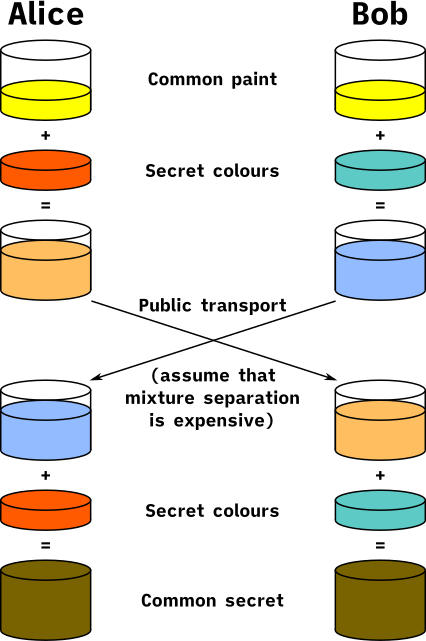
\includegraphics[width=.8\textwidth]{slides/security-fundamental-concepts/Diffie-Hellman_Key_Exchange.pdf}\\
      \scriptsize Diffie-Hellman key exchange analogy\\
      \tiny A.J. Vinck, Public domain: \\\url{https://en.wikipedia.org/wiki/File:Diffie-Hellman_Key_Exchange.svg}\\
    \end{center}
  \end{columns}
\end{frame}

\subsubsection{Real world use cases}

\begin{frame}
  \frametitle{Symmetric vs asymmetric cryptographic algorithms}
  \begin{itemize}
    \item Symmetric and asymmetric cryptographic algorithms tend to have opposite
      advantages:
      \begin{itemize}
        \item Symmetric algorithms:
          \begin{itemize}
            \item Low RAM and CPU requirements
            \item Can easily be hardware accelerated
            \item Requires a previously and secretly exchanged key between each
              pair of peers
          \end{itemize}
        \item Asymmetric algorithms:
          \begin{itemize}
            \item Hardware resources hungry
            \item Each peer needs to publish only one public key.
          \end{itemize}
      \end{itemize}
    \item In practice, most protocols will rely on a combination of symmetric and
      asymmetric algorithms.
  \end{itemize}
\end{frame}

\begin{frame}
  \frametitle{Typical use cases}
  \begin{itemize}
    \item Some use cases will only need to sign data:
      \begin{itemize}
        \item RSA, ECDSA, or EdDSA can be used
        \item Typical example: secure boot
      \end{itemize}
    \item Some use cases will only need to encrypt data:
      \begin{itemize}
        \item AES can be used with an appropriate block cipher mode of operation
        \item Typical example: disk encryption
      \end{itemize}
    \item Secure communication protocol will use a mix of all of these:
      \begin{itemize}
        \item RSA, ECDSA, or EdDSA for authentication
        \item DH of ECDH for key exchange
        \item AES for communication once the secure connection is established
        \item Typical protocols: TLS, SSH, GPG…
      \end{itemize}
  \end{itemize}
\end{frame}

\subsection{Understanding a TLS handshake}

\begin{frame}
  \frametitle{The Transport Layer Security Protocol}
  \begin{itemize}
    \item First proposed in 1999 by the IETF as the Secure Sockets Layer (SSL)
      protocol
    \item Allows servers and clients to communicate in a secure way:
      \begin{itemize}
        \item Authenticate the peers, either server-only or both ends
        \item Encrypt connection to prevent eavesdropping
      \end{itemize}
    \item It relies on several cryptographic mechanisms, including public-key
      and symmetric encryption.
    \item Relies on public key certificate to verify the remote public key
  \end{itemize}
\end{frame}

\begin{frame}
  \frametitle{Understanding the TLS protocol}
  \begin{itemize}
    \item TLS protocol is based on \emph{records} containing either protocol
      management data or application data.
    \item Two main phases:
      \begin{itemize}
        \item A handshake phase:
          \begin{itemize}
            \item The algorithms to use during the session are selected
            \item Peers are authenticated
            \item Session keys are exchanged
          \end{itemize}
        \item A data exchange or ``Application'' phase
      \end{itemize}
    \item This is a highly simplified view: application records can be
      interleaved with connection management records, such as key renegotiation or
      alerts.
  \end{itemize}
\end{frame}

\begin{frame}
  \frametitle{TLS handshake with server authentication only}
  \begin{columns}
    \begin{column}{0.7\textwidth}
      \begin{itemize}
        \item<1-> Assumptions
          \begin{onlyenv}<1>
            \begin{itemize}
              \item Only the server is authenticated
              \item This is the first time the peers connect
              \item TLS version 1.3: \url{https://www.rfc-editor.org/rfc/rfc8446}
            \end{itemize}
          \end{onlyenv}
        \item<2-> Client: Client Hello
          \begin{onlyenv}<2>
            \begin{itemize}
              \item Very first message, sent by the client willing to open the connection
              \item Contains:
                \begin{itemize}
                  \item The client protocol version
                  \item A 32 bytes random number
                  \item The list of supported symmetric cipher suites (e.g., \texttt{AES\_128\_CCM}, \texttt{CHACHA20\_POLY1305})
                  \item A list of supported mechanisms for key exchange and their associated
                    values (e.g., Diffie-Hellman with client public parameters).
                \end{itemize}
            \end{itemize}
          \end{onlyenv}
        \item<3-> Server: Server Hello
          \begin{onlyenv}<3>
            \begin{itemize}
              \item Server reply agreeing on the configuration to use
              \item Contains:
                \begin{itemize}
                  \item The selected protocol version (e.g., TLS 1.3)
                  \item A 32 bytes random number
                  \item The selected symmetric cipher suites, e.g. \texttt{AES\_128\_CCM}
                  \item One of the key exchange mechanisms offered by the client and its
                    associated values (e.g., Diffie-Hellman with server public parameters).
                \end{itemize}
            \end{itemize}
          \end{onlyenv}
        \item<4-> Server: Certificate
          \begin{onlyenv}<4>
            \begin{itemize}
              \item Provides the server certificate
            \end{itemize}
          \end{onlyenv}
        \item<4-> Server: Certificate Verify
          \begin{onlyenv}<4>
            \begin{itemize}
              \item Provides a proof the server owns the corresponding private key
              \item Contains:
                \begin{itemize}
                  \item A signature of all previous handshake messages
                \end{itemize}
              \item Algorithms depend on the certificate, e.g. ECDSA
            \end{itemize}
          \end{onlyenv}
        \item<5-> Server: Finished
          \begin{onlyenv}<5>
            \begin{itemize}
              \item Confirms the handshake step is done from the server side: the client
                can now send Application data
              \item Contains:
                \begin{itemize}
                  \item A MAC covering the entire handshake (using an HMAC algorithm)
                \end{itemize}
            \end{itemize}
          \end{onlyenv}
        \item<6-> Client: Finished
          \begin{onlyenv}<6>
            \begin{itemize}
              \item Confirms the handshake step is done from the client side: the server
                can now send Application data
              \item Contains:
                \begin{itemize}
                  \item A MAC covering the entire handshake (using an HMAC algorithm)
                \end{itemize}
            \end{itemize}
          \end{onlyenv}
        \item<7-> Application data can then be sent between peers
          \begin{onlyenv}<7>
            \begin{itemize}
              \item Algorithm and operation mode has been selected during the handshake,
                e.g. \texttt{AES\_128\_CCM}
              \item Key has been constructed from the key exchange data during the
                handshake
            \end{itemize}
          \end{onlyenv}
      \end{itemize}
    \end{column}
    \begin{column}{0.3\textwidth}
      \includegraphics<1>[width=\textwidth]{slides/security-fundamental-concepts/tls_empty.pdf}
      \includegraphics<2>[width=\textwidth]{slides/security-fundamental-concepts/tls_client_hello.pdf}
      \includegraphics<3,4,5>[width=\textwidth]{slides/security-fundamental-concepts/tls_server_finish.pdf}
      \includegraphics<6>[width=\textwidth]{slides/security-fundamental-concepts/tls_client_finish.pdf}
      \includegraphics<7>[width=\textwidth]{slides/security-fundamental-concepts/tls_full.pdf}
    \end{column}
  \end{columns}
\end{frame}


\subsection{Understanding Public Key Infrastructures}

\begin{frame}
  \frametitle{Public key certificate}
  \begin{itemize}
    \item Certifies that a specific public key is assigned to a specific entity
    \item Is signed by a certificate authority (CA)
    \item Certificate signature can then be verified by the CA own certificate
      \begin{itemize}
        \item This creates a chain of trust extending to a root certificate
        \item Root certificates are not guaranteed by a third-party: they have to be
          known by the client
      \end{itemize}
    \item The certificate has to follow a specific format, quite often ITU-T X.509
      is used
    \item Certificates can generally be revoked: this information is not presented
      by the certificate itself but has to be retrieved by other means
  \end{itemize}
\end{frame}

\begin{frame}
  \frametitle{Public key certificate content}
  \begin{itemize}
    \item Content of the certificate will depend on its goal and the CA policy
    \item Common content:
      \begin{itemize}
        \item A subject: which entities this certificate belongs to. This may be
          a machine, an individual, or an organization
        \item A serial number, allowing one to uniquely identify each
          certificate
        \item The period of validity
        \item The purpose of the certificate: authenticate the entity for a specific
          service or a specific operation
        \item The public key
        \item The issuer (CA) and its signature
      \end{itemize}
  \end{itemize}
\end{frame}

\begin{frame}
  \frametitle{Public key infrastructure}
  \begin{itemize}
    \item Certificates should be assigned to each entities, allowing them to
      authenticate to their peers
    \item These certificates should be signed by a certificate authority and
      issued to legitimate users
    \item The Public key infrastructure defines the organisation and processes
      governing these certificates
    \item PKI use case examples:
      \begin{itemize}
        \item Establishing TLS connections, e.g.\ over HTTP
        \item Authenticate and encrypt e-mail messages, e.g.\ with openPGP
        \item Authenticate devices in a fleet, where the PKI is entirely managed
          by the device vendor
      \end{itemize}
  \end{itemize}
\end{frame}
